\chapter{Android系统相关背景介绍 }  
\label{ch2}


本章首先会简要介绍Android系统架构,其次会对Android中的Activity组件做基本介绍,接着会着重介绍Android中常见的两种多线程交互方式,最后将指出本文系统在实现上的难点。

\section{Android系统结构介绍}

Android是基于Linux内核开发的的开源操作系统,隶属于Google公司,主要用于触屏移动设备如智能手机、平板电脑与其他便携式设备,是目前世界上最流行的移动终端操作系统之一。

在系统架构上,Android自下到上,可以分为四层:Kernel层、Library和Android Runtime(Dalvik/ART)、Framework、Application等,如~\autoref{fig:Android-Framework}所示。
Kernel层是硬件和软件层之间的抽象层,主要是设备的驱动程序,例如:显示驱动、音频驱动、蓝牙驱动、Binder IPC驱动等。
Library和Android Runtime(Dalvik/ART): Library,顾名思义就是向上层提供各种这样的基础功能,例如SQLite数据库引擎,Surface Manager显示系统管理库。
Android Runtime主要是运行Android程序的虚拟机,在不同版本的系统上对应着不同的虚拟机,例如在Android 5.0及以上是ART,而在Android 4.3及以下是Dalvik,而Android 4.4两者都有。
Framework层主要是系统管理类库,包括Activity的管理,消息通知的管理;同时,它是Application的基础架构,为应用程序层的开发者提供了API,其存在简化了程序的开发。
而Application就是我们平时接触的应用,开发人员公国调用底层Framework提供的API实现相应的接口。

虽然Android应用程序是使用Java语言开发的,但是它和传统的Java程序有着很大的不同,具体有如下几点:

\begin{figure*}
	\centering
	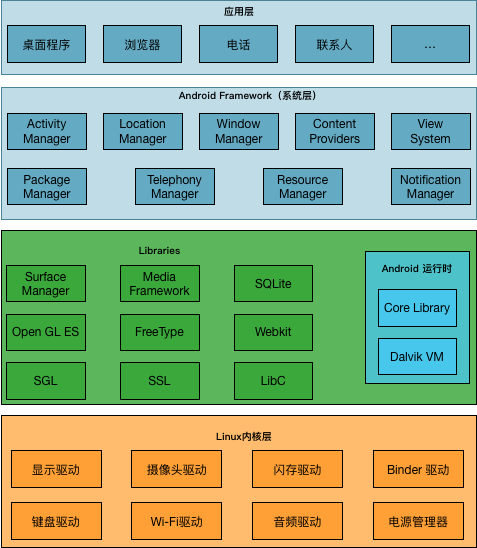
\includegraphics[width=\textwidth]{./Figures/Android-Framework.png}
	\caption{Android系统框架图}
	\label{fig:Android-Framework}
\end{figure*}


\textbf{异于常规程序的开发方式:}
在设计上,Android应用程序的开发架构采用的是事件驱动架构。在开发过程中,没有传统程序中入口函数Entry Point的概念。应用程序中通用的业务逻辑(例如应用程序如何启动退出、应用的窗口如何创建销毁等)存在于Android Framework中。这也使得Android应用程序的分发文件(即APK文件)相对较小。

\textbf{面向组件的开发方式:}
Android程序中较为常见的是组件(Component,例如Activity、Service、Content Provider、Broadcast Receiver),它是应用程序运行的最小单元,受到Android Framework的直接调度。开发人员通过继承这些组件,重写对应的生命周期函数,已实现对应的业务需求(界面的布局、页面状态的保存等),而这些组件的生命周期由Framework调度完成。

\textbf{大量逻辑实现依赖于回调函数和多线程通信:}
由于Android应用程序采用的是基于单线程消息队列的事件驱动架构,因此,界面相关的操作只允许出现在主线程(UI Thread)中,耗时操作只能在工作线程(Worker Thread)中进行。通常的,开发人员往往会借助回调函数处理控件的响应事件,利用多线程交互串联界面相关操作和耗时操作,完成对应的业务。


\section{Android中的Activity}

在Android应用程序运行过程中,Activity向用户展示图形界面,响应用户的反馈,和其他组件一同完成相关业务,扮演着最为重要的作用。由于Android应用程序在架构选型上采用了事件驱动模型,为了便于协调应用内部状态的管理,Android组件通常有生命周期的概念,Activity也不例外。

Android系统根据Activity 在运行时和用户的反馈将其状态分为以下四种:
\begin{enumerate}

\item 运行态:在该状态下, Activity处于页面最前端时,用户可以与Activity进行交互。一般的,我们看到Activity均处于这个状态。

\item 暂停态:在该状态,Activity仍然可见,但是失去了窗口的焦点。当一个Activity之上出现一个透明的Activity、Toast或者对话框时,Activity就处于这个状态。处于暂停状态的Activity仍处于存活状态,保存着所有的内存数据,只有当系统内存极度紧张时,才有可能被系统杀死回收。

\item 停止态:当一个Activity被其他的Activity遮挡时,处于这个状态。处于该状态的Activity仍然可以保留所有的状态,只是对用户不可见。系统在需要内存的情况下,可以采用相应的策略对Activity进行杀死回收操作。

\item 终止态:当Activity处于暂停态或者停止态时,系统由于内存原因可能会将上述两种Activity杀死回收。处于该状态下的Activity将不能直接恢复。
\end{enumerate}

Activity的生命周期就是以上状态之间的跳转,受到Activity在运行时的内存分布、环境状态以及业务逻辑的影响,由Android系统直接负责调度。
Android系统为Activity提供了onCreate(), onStart(), onResume(), onPaused(), onRestart(),  onStoped()和onDestroy()等方法,方便开发人员在Activity的状态发生变化时对程序的运行时数据和应用状态做适当的处理操作。对应的Activity的生命周期具体如~\autoref{fig:Activity-lifecycle}所示:

 
\begin{figure*}
	\centering
	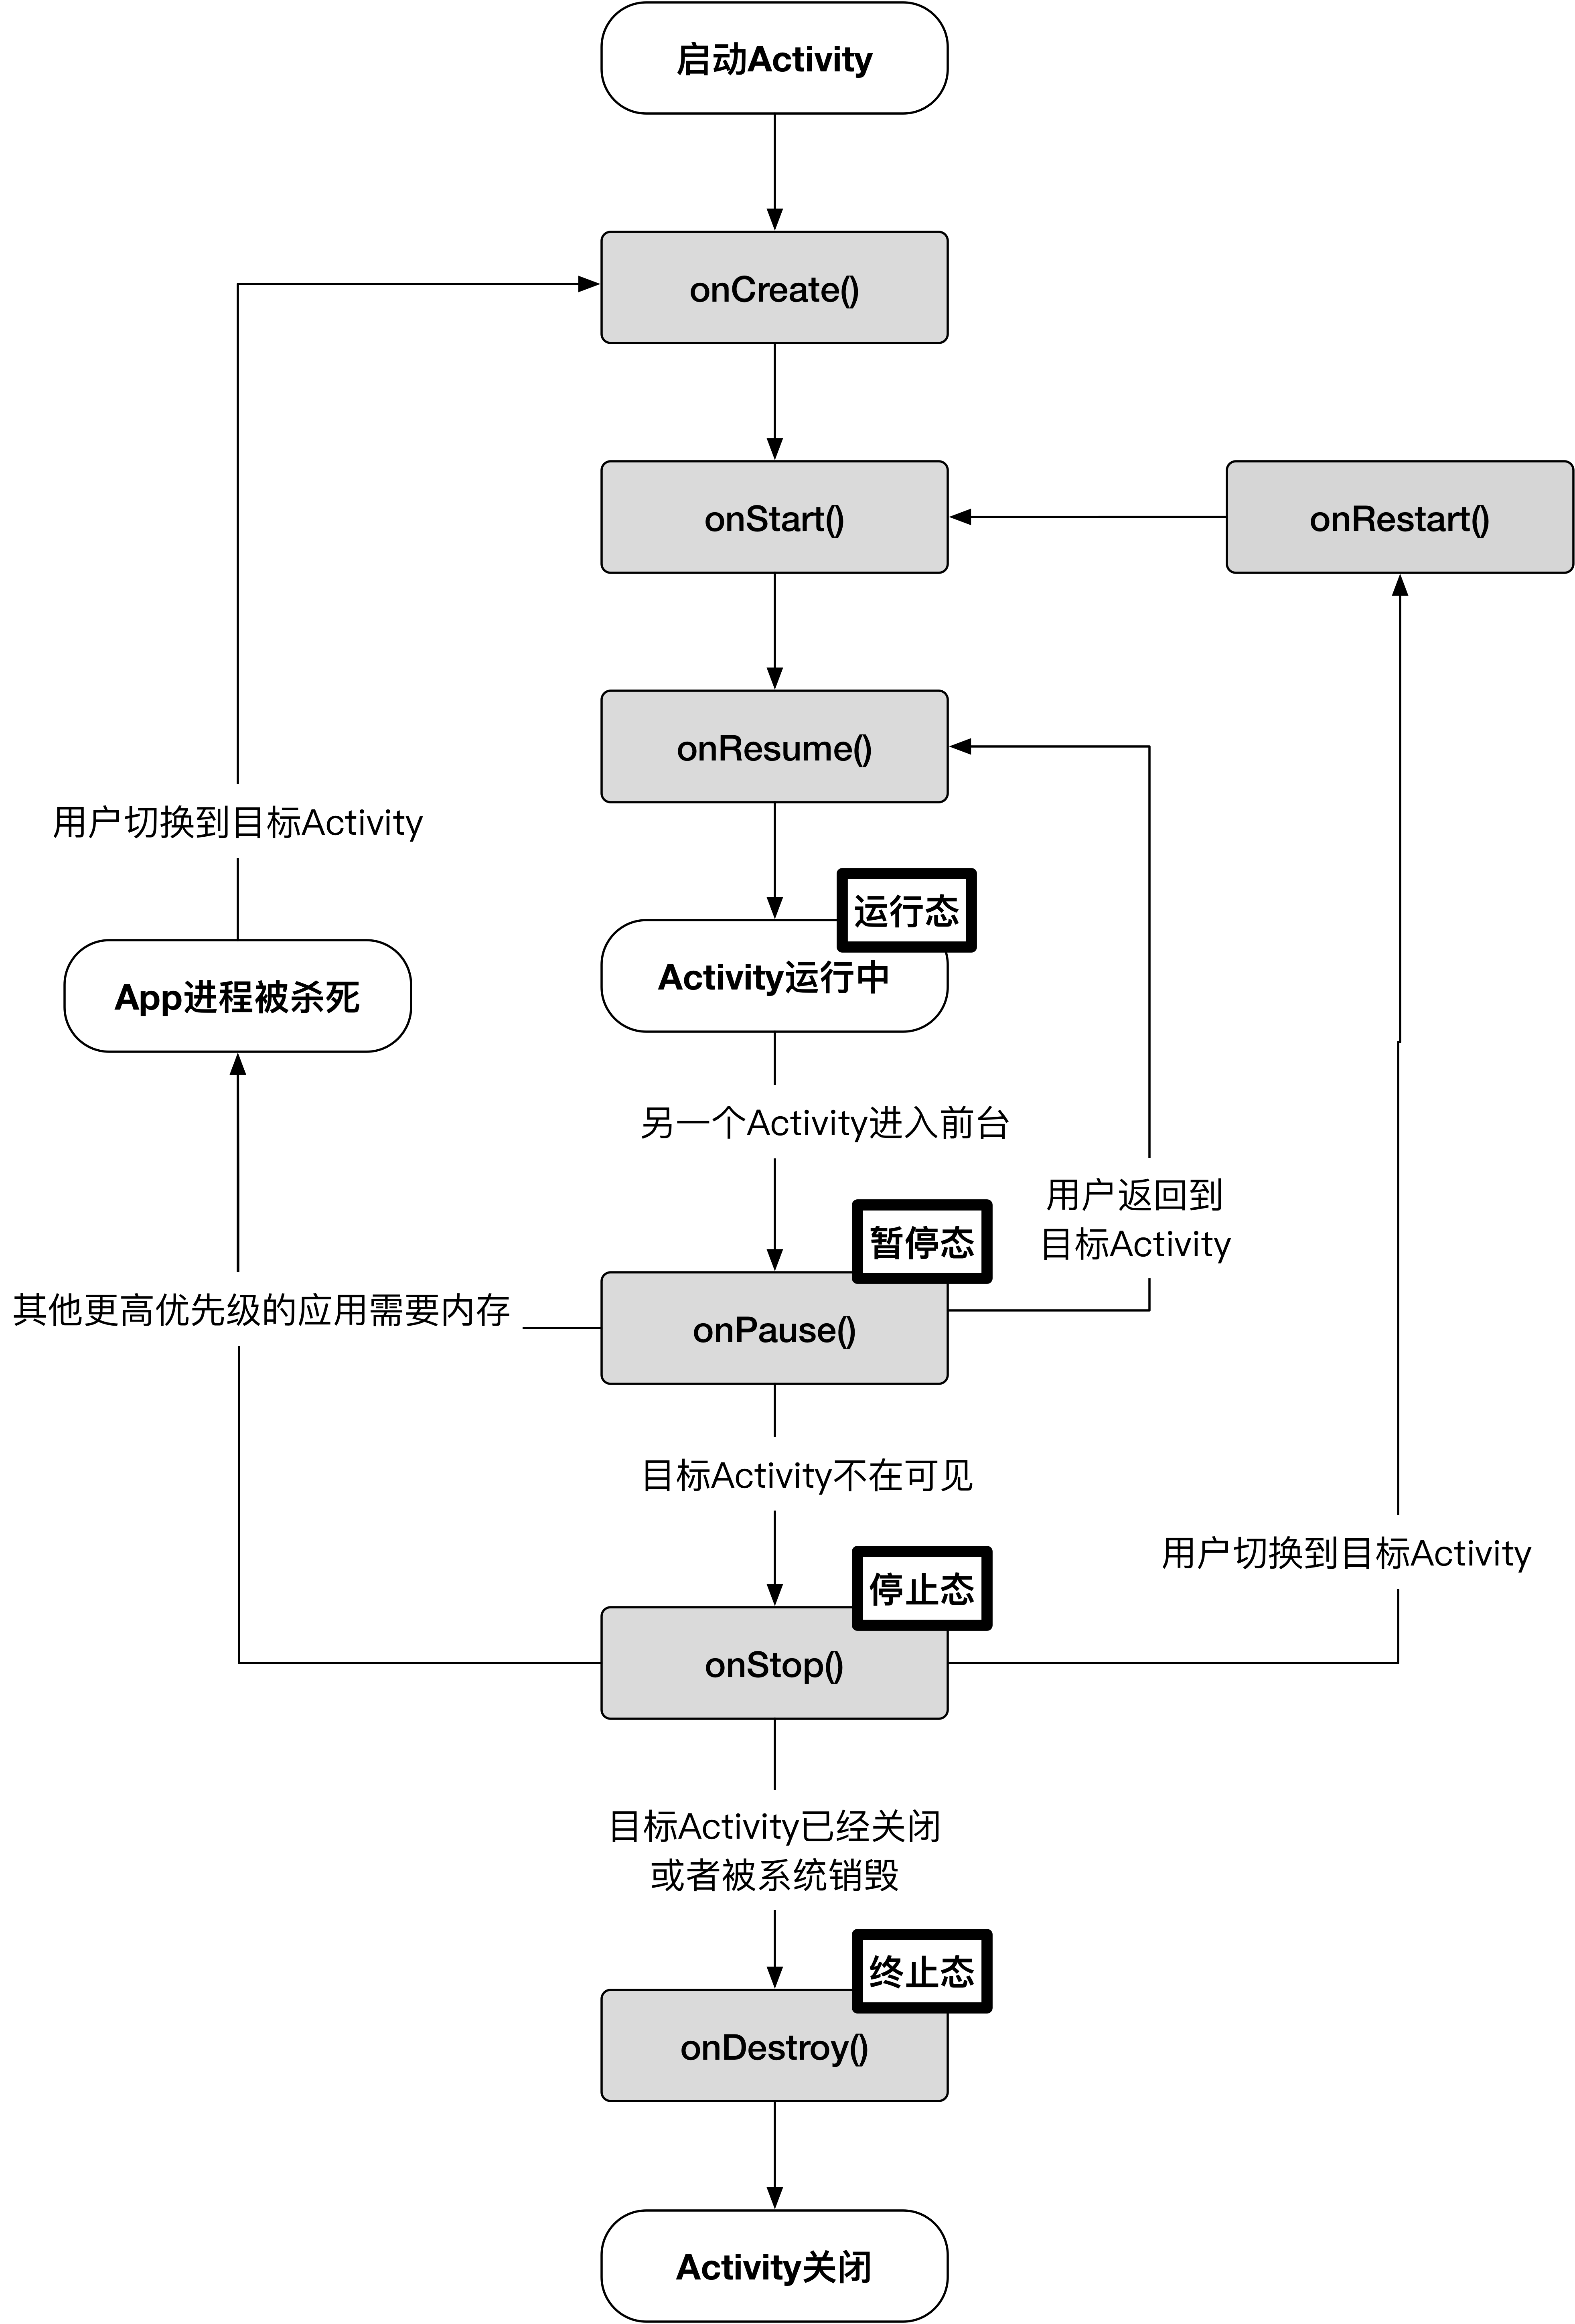
\includegraphics[width=\textwidth]{./Figures/Activity-lifecycle.png}
	\caption{Activity的生命周期}
	\label{fig:Activity-lifecycle}
\end{figure*}


当用户点击应用图标,系统启动应用程序后,系统会创建Activity、启动Activity并使之可以和用户进行交互,在这个过程中,onCreate()、onStart()、onResume()等方法被回调,Activity最终处于运行态;

当用户点击“返回键”返回到桌面时,Activity会失去焦点,在用户的视野中消失,直至被系统回收,对应的状态也从运行态经暂停态、停止态,变为终止态变,期间onPause()、onStop()、onDestroy等方法被回调;

当用户从一个界面回到原来的界面时,原有的Activity从停止态重启,先后出现在设备界面上,获得和用户交互的焦点,期间onRestart()、onStart()、onResume()等方法被回调;

当一个Activity长期处于停止态,但由于内存原因被系统回收时,用户尝试启动它时,系统会像启动一个新的Activity一样启动它。

\section{Android中的多线程交互}
 Android系统在架构设计上采用了事件驱动架构。在多线程并发访问时,若UI控件对于各线程均是可见的,并发对控件做读写操作会使控件处于不可预期的状态;若贸然对控件使用锁机制,这将会使阻塞部分线程业务逻辑的执行,使得应用变得复杂低效。上述情况对于应用程序都是不可接受的。为了避免多线程操作之间的竞争关系带来的低效率问题,Android系统在设计事件驱动架构时,采用了单线程的消息队列,即只允许在主线程(也称为主线程,Main Thread)进行界面更新操作,不允许在其他线程(也称为工作线程,Worker Thread)进行界面更新操作。

当应用程序出现耗时操作(例如加载磁盘上的图片、网络请求等)时,应用程序往往需要在一个新的线程中执行上述逻辑。当应用程序界面中的某些控件需要根据耗时操作的结果(例如渲染得到的图片对象、网络请求得到的JSON字段)更新界面状态时,开发人员需要切换到主线程进行界面的更新。

从整体上,开发者可以需要的交互方式分为基于Java的多线程交互和基于Handler的交互方式。

\subsection{基于Java的多线程交互}

由于Android系统提供的API接口兼容Java多线程相关的部分API,因此,在Android系统中,开发人员可以采用和Java应用相同的调用方式启动工作线程,并在对应的线程上完成业务逻辑。但是,Java API只能实现业务逻辑从原有线程转移到新的工作线程上,不能重新返回到主线程上。为此,Android系统在Java API的基础上还提供了void runOnUiThread (Runnable action) API。runOnUiThread API可以帮助开发人员将业务逻辑的执行从工作线程转移到主线程上,该API也符合Android只允许在主线程上更新界面这一基本设计原则。但是,该API也存在着一些弊端,例如runOnUiThread API的定义位于类android.app.Activity,这也就意味着在Android组件Service中进行耗时操作时,无法通过该API返回到主线程;同时基于接口的函数参数定义方式对于跨线程的参数传递也不是十分友好。为此,Android提供了基于Handler的多线程交互方式。

\subsection{基于Handler的多线程消息调度}

为了满足开发人员多样化的业务在多线程间的切换,Android提供了基于Handler消息调度的多线程交互方式。当开发人员需要当前业务逻辑转移到其他线程时,通过方法Message.obtain()获取一个Message,将对应的业务逻辑封装成Runnable对象传递给Message中对应的字段,或者将对应的参数传递给Message中的参数字段,最后通过Handler对象发送给指定的消息队列。当目标线程的消息队列读取到这条消息时,便会在该线程中执行预定的业务逻辑。

~\autoref{fig:handler-code}为Handler的简单示例:用户在工作线程执行一项耗时任务(生成一个字符串),将生成的字符串传递给Message对象,并通过Handler对象通知主线程进行界面更新。
 
 
\begin{figure*}[h]
	\centering
	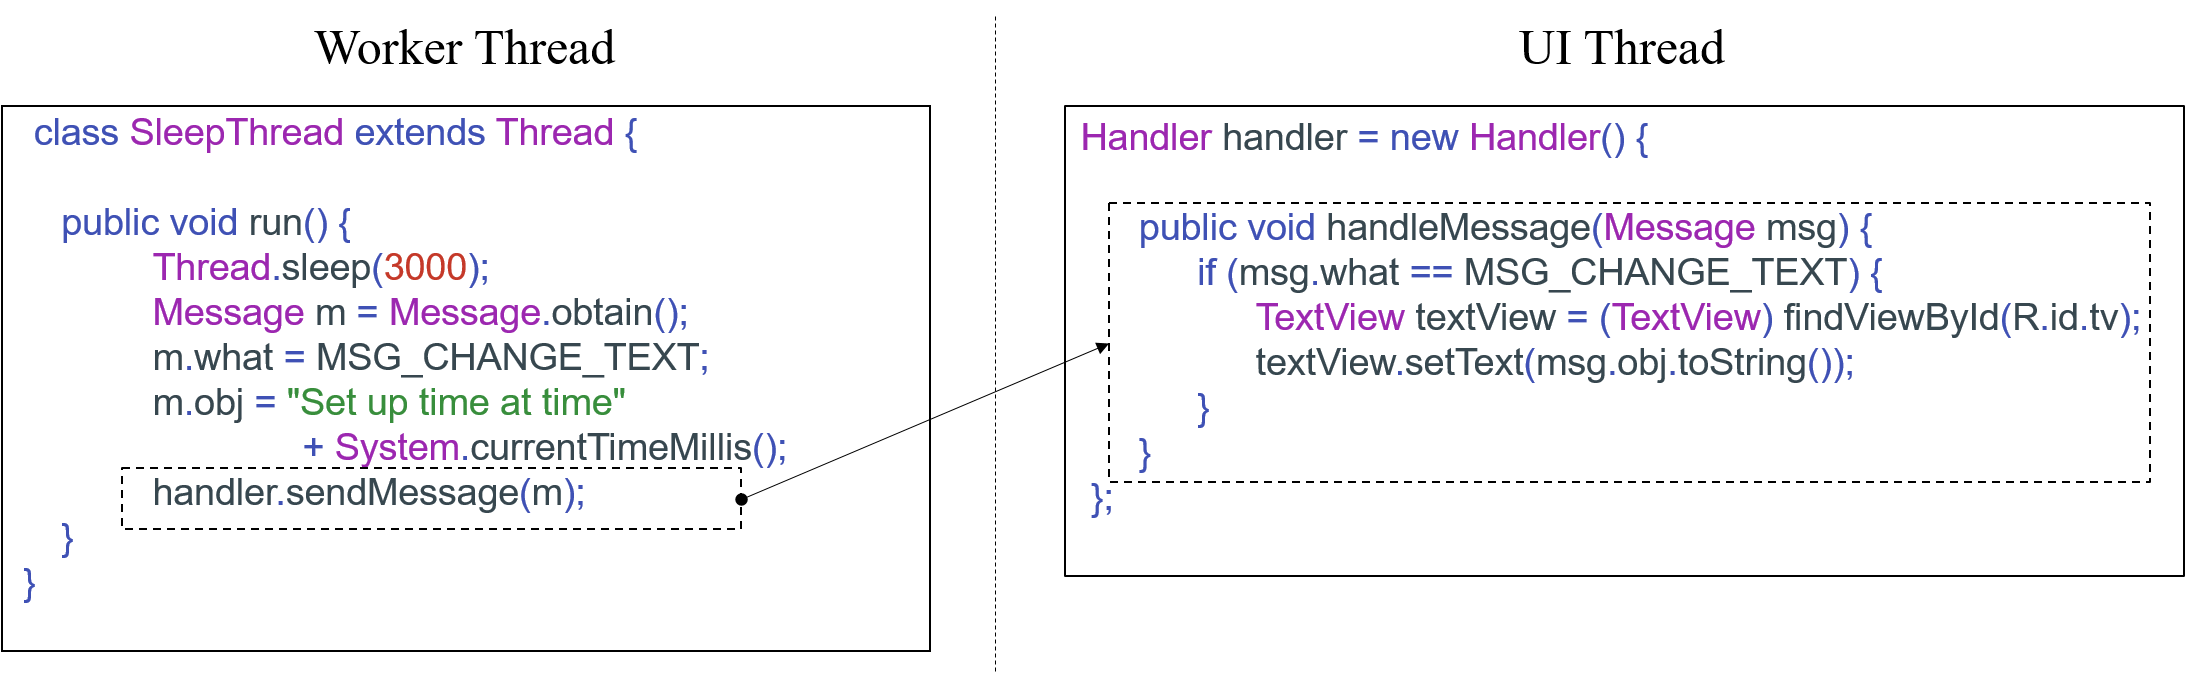
\includegraphics[width=\textwidth]{./Figures/handler-code.png}
	\caption{Handler的使用实例}
	\label{fig:handler-code}
\end{figure*}


从Android SDK提供的API来看,开发人员可以通过post(Runnable),postAtTime(Runnable,long),sendMessage(Message),postDelayed(Runnable, Object, long), sendMessageDelayed(Message,long),sendMessageAtTime(Message,long)和sendEmptyMessage(int)等多种API形式实现消息调度。通过查阅和分析Android系统相关源代码,我们发现上述Handler相关的API关系如~\autoref{fig:handler-apis}所示。

 
 \begin{figure*}[h]
	\centering
	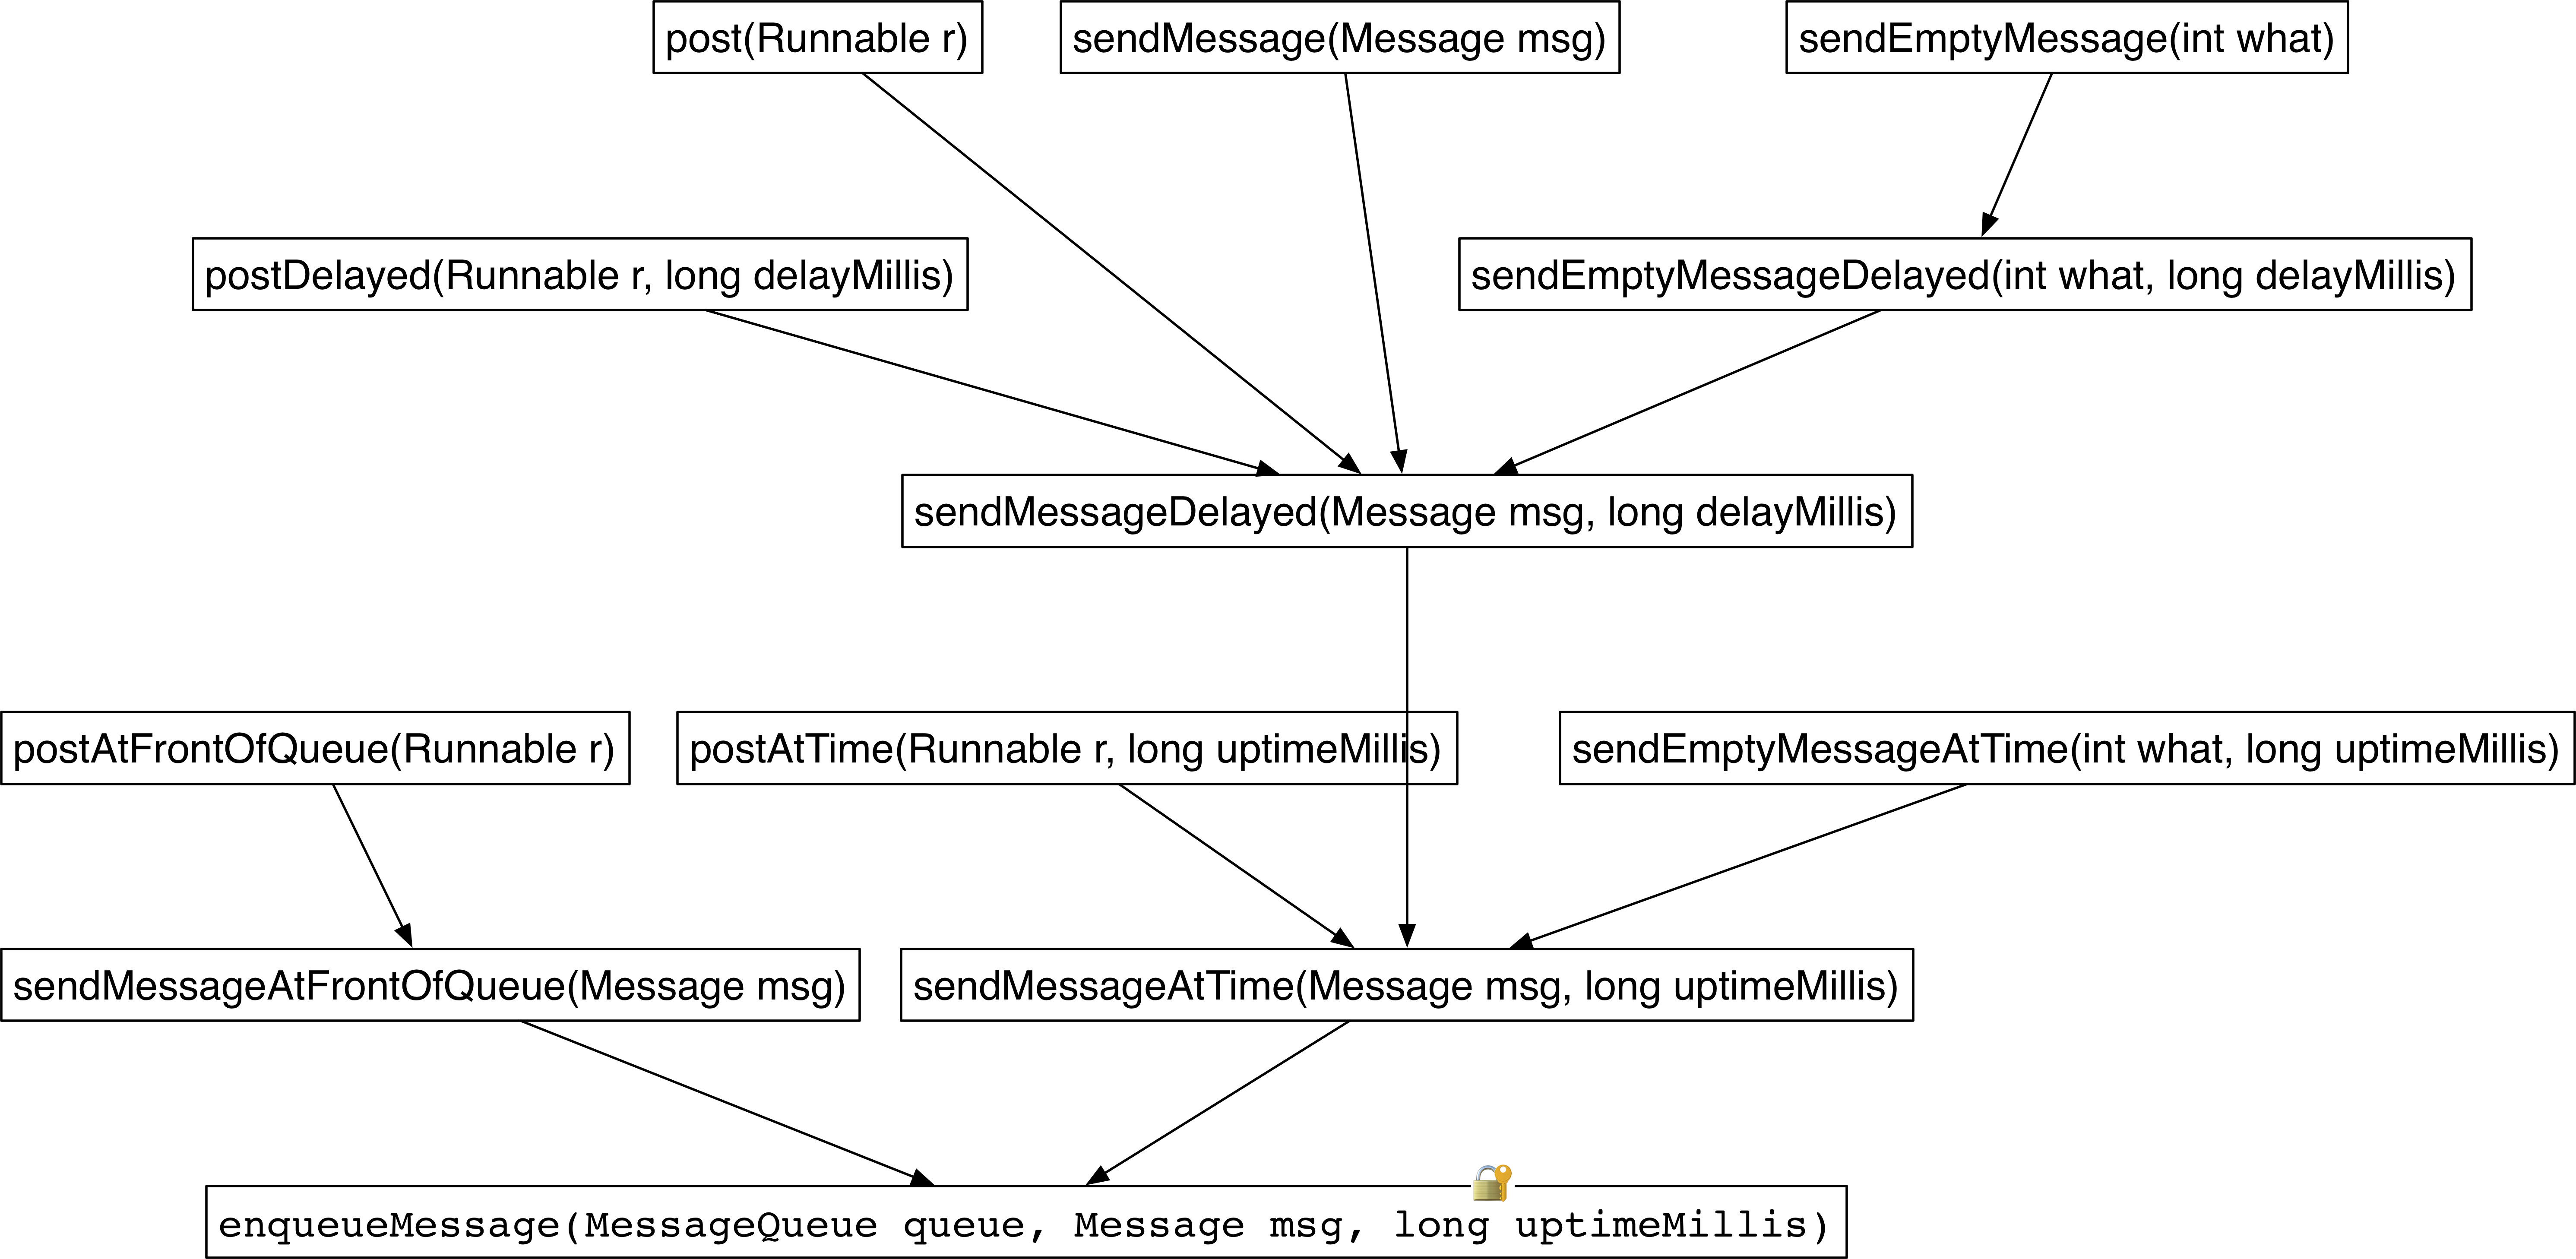
\includegraphics[width=\textwidth]{./Figures/Handler-apis.png}
	\caption{ Handler 各API之间的调用关系}
	\label{fig:handler-apis}
\end{figure*}


从~\autoref{fig:handler-apis}中,我们可以发现所有的API最后就会调用到android.os.Handler enqueueMessage(MessageQueue, Message, long)方法。

从底层实现上看,Handler机制主要由Handler、Looper、MessageQueue、Message等若干部分组成。Message是跨线程交互的主要载体,Android系统采用对象池的设计模式来管理Message对象;无论开发人员以何种形式调用了Handler发送消息,传递的参数最后均会封装到Message对象中。MessageQueue则存放着所有待处理的Message对象,它是一个双端队列,开发人员可以根据具体业务场景在消息队列的头部、尾部或者适当位置插入消息队列。Looper则负责以epoll的方式从MessageQueue中循环读取Message对象,分发给对应的Handler对象使得业务可以在对应恰当的线程上被处理;一个线程最多只允许只有一个Looper对象,他只能绑定一个与之对应的MessageQueue;其中最为常见的就是位于主线程的MainLooper,它主要负责Android系统的日常调度(例如Activity的生命周期、控件的点击事件响应等)。Handler对象则负责将消息发送到对应的MessageQueue中(扮演着消息的生产者角色)以及消费来自Looper分发下来的Message(扮演着消息的消费者角色);在一个应用中,Handler可以存在多个对象,一个Handler对象也可以同时扮演生产者和消费者两个角色。

从原理上看,基于Handler的多线程消息调度,充分利用了Android的事件驱动架构,将业务逻辑抽象出Message对象。该消息对象通过Handler的对应接口发送至在目标线程所对应的消息队列MessageQueue中,再由Looper对象在目标线程运行时从消息队列中取出,分发给对应的Handler执行,达到了Android跨线程交互的目的。具体地,Handler的工作原理如~\autoref{fig:handler-framework}所示:
 

 \begin{figure*}[h]
	\centering
	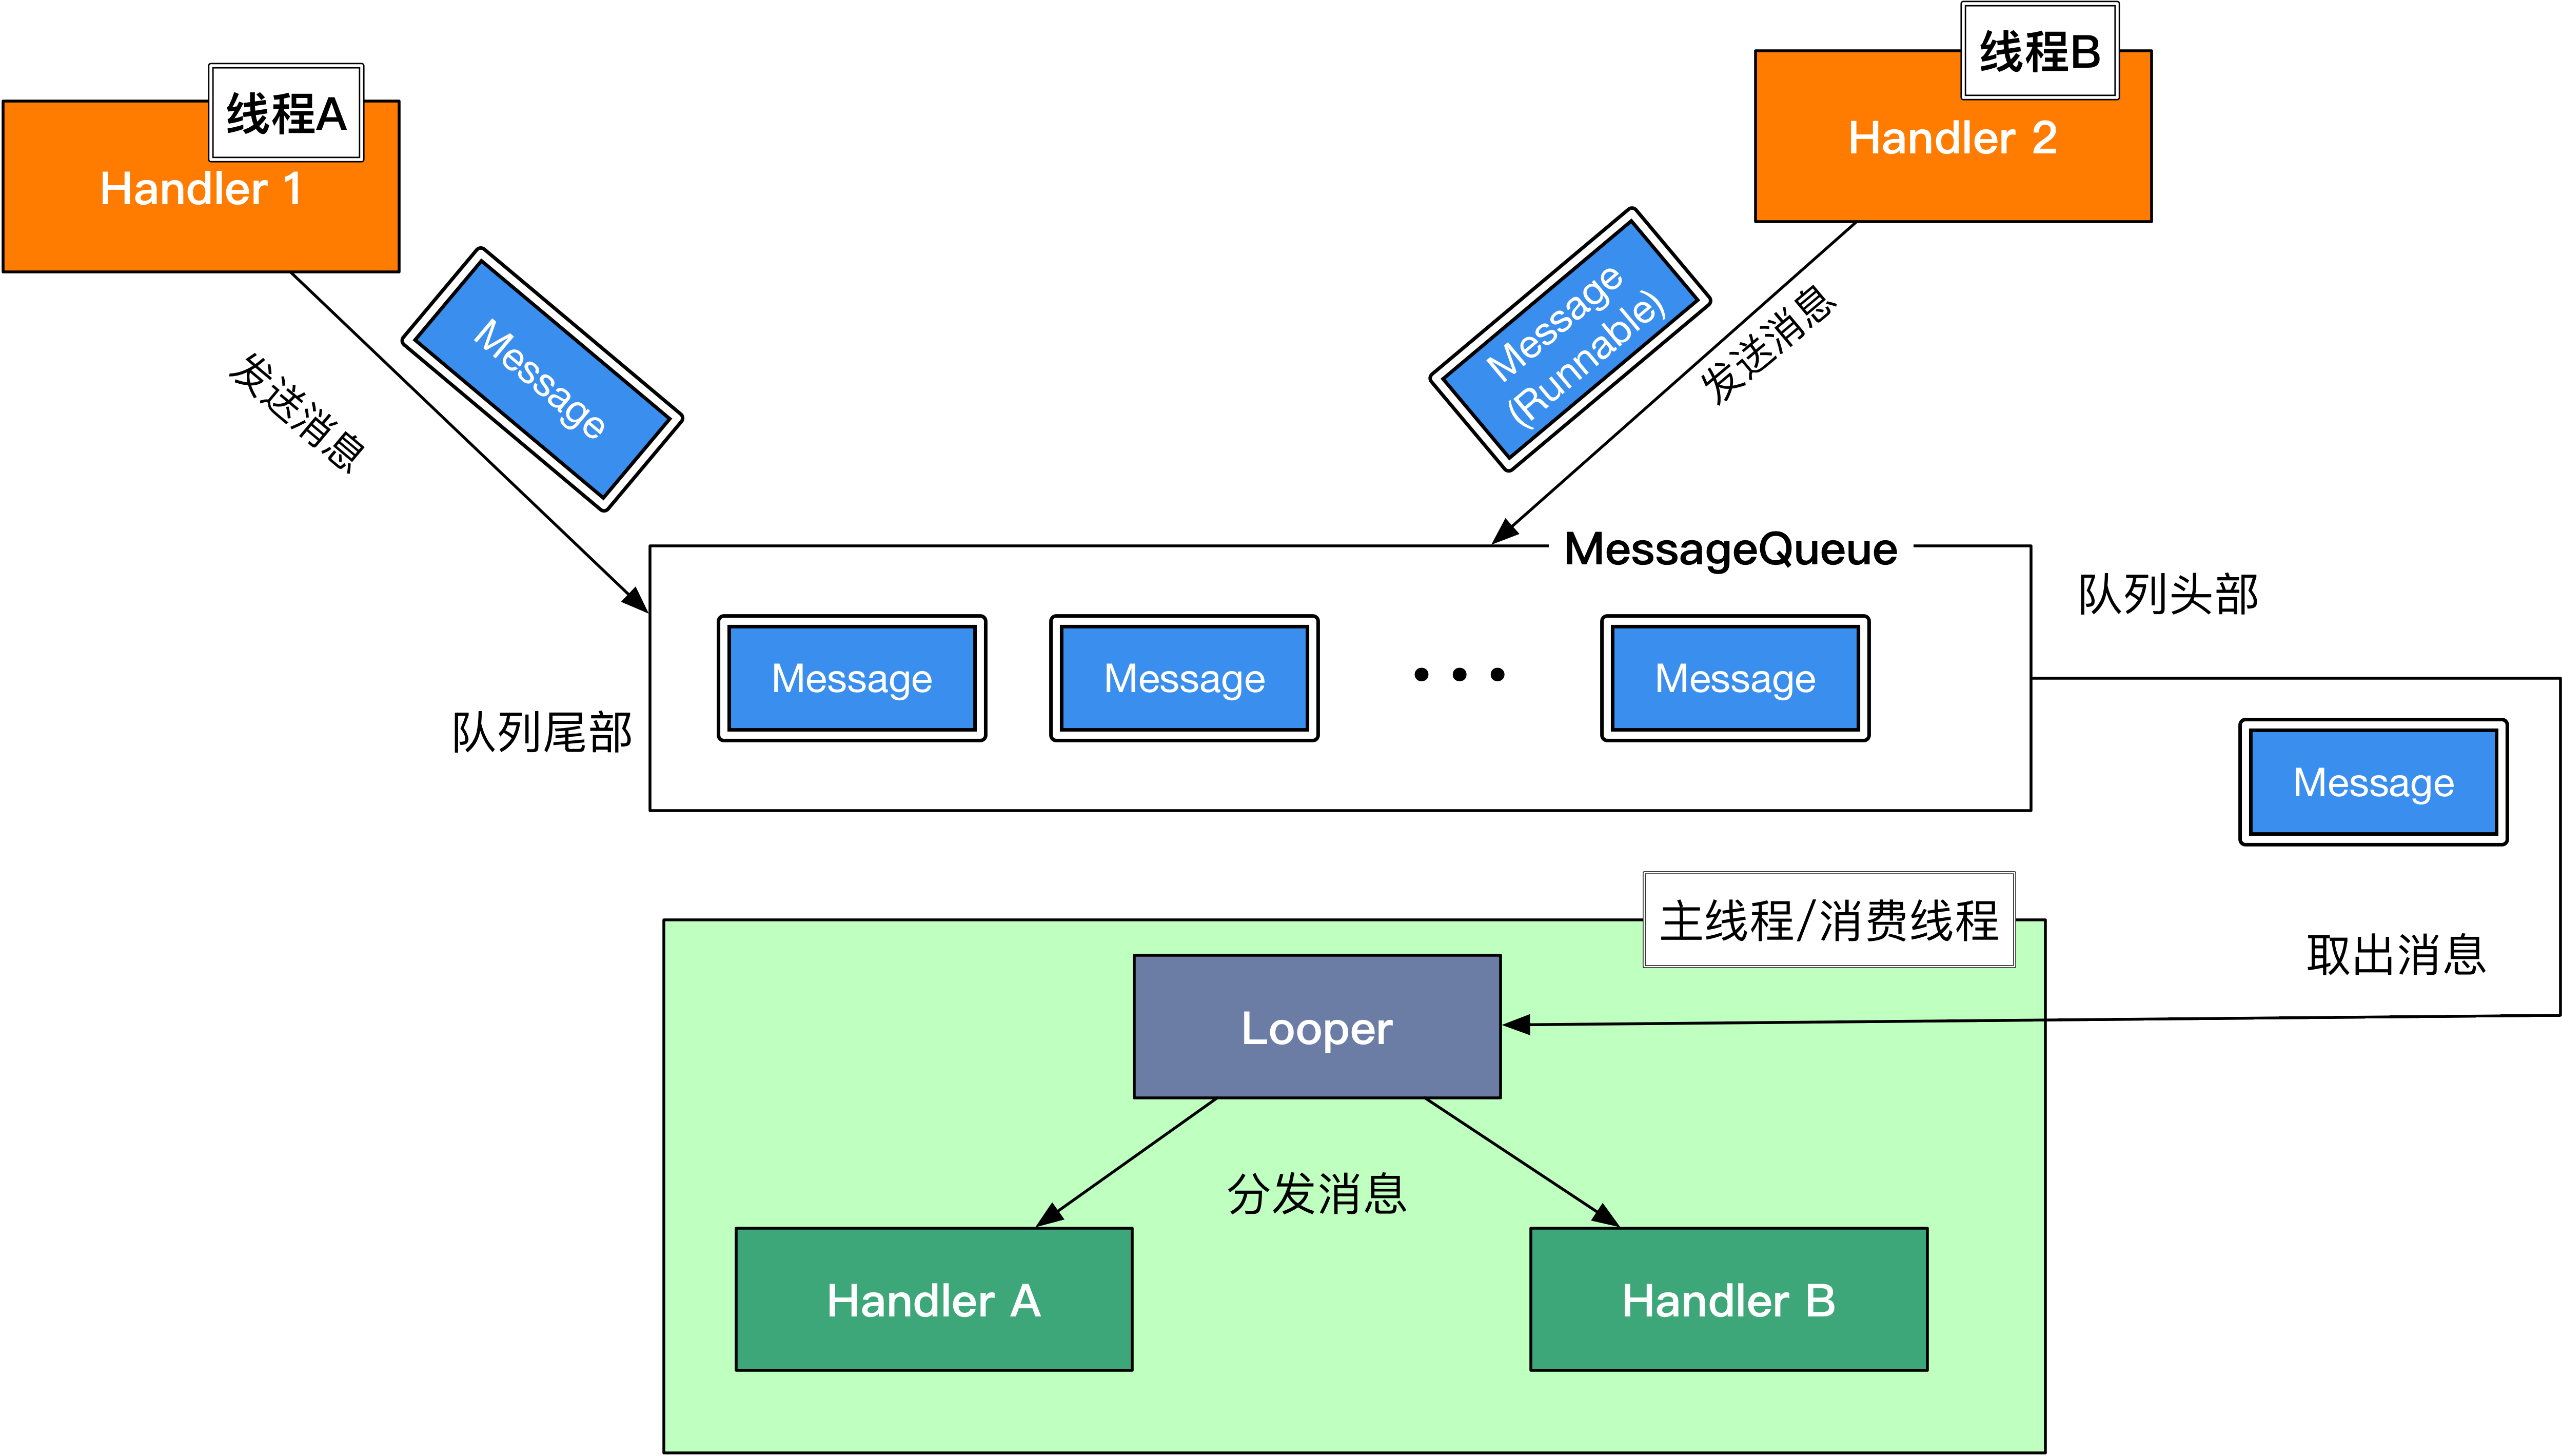
\includegraphics[width=\textwidth]{./Figures/Handler-framework.png}
	\caption{ Handler的工作原理}
	\label{fig:handler-framework}
\end{figure*}


综上所述,基于Handler消息调度的多线程交互方式,不仅可以帮助开发人员实现业务逻辑在主线程和工作线程间的自由转移,而且其灵活的API设计还帮助开发人员降低应用的设计复杂程度,提升了系统架构的可拓展性。因此,在Android开发过程中,基于Handler消息调度的多线程交互十分常见。
\section{本文遇到的困难与挑战}


 本文解决的关键问题有如下几点:

1)	如何获取应用程序中各个函数的执行信息?

获取应用程序在执行过程中各函数执行信息是本文的基础。从函数分类上,用户定义的方法和系统预定义的方法。对于前者,我们可以通过修改程序源代码实现;但对于后者,由于我们无法直接修改系统程序的源代码或者构建一个符合本文业务需求的系统的成本较高,为此,我们需要寻找对应的解决方案以帮助我们获取系统方法的执行信息。

2)	如何根据程序中各函数的的执行信息,还原应用程序的函数调用图?

基于第一点,我们可以获取程序在运行过程中的执行信息。但仅仅依靠这些执行信息是不够的,我们还需要将这些执行信息组织起来,挖掘执行信息之间的关联关系,从而才能还原成应用程序的函数调用图。这将是本文研究的重点之一。

3)	如何在生成的函数调用图中体现Android特性?

正如上文所提的,Android系统中有很多常规应用中不具备的特性,例如Activity的生命周期、基于多线程调用的触发关系。若要在生成的函数调用图上体现上述特性,需要对Android系统源代码有一定的了解熟悉,并基于图中的相关信息创建与特性相对应的关系,这既是本文研究的重点,也是本文的创新点。

\section{本章小结}

本章主要介绍了Android系统的相关背景知识,较为详细的阐述了Android的系统结构,详细介绍了Android四大组件之一的Activity机器生命周期。同时,本章还介绍了基于Runnable/Thread、Handler消息调度两种不同的多线程交互方式,较为详细地分析了Handler的运行机制,为下文基于函数调用图的多线程触发关系生成做了铺垫。最后,本章还介绍了系统在实现上可能遇到的困难。
